% Preview source code

%% LyX 2.1.4 created this file.  For more info, see http://www.lyx.org/.
%% Do not edit unless you really know what you are doing.
\documentclass[12pt,oneside,english,american,oldfontcommands]{memoir}

%%% packages used
\usepackage{mathptmx}
% \usepackage{mathpazo} % palatino
\renewcommand{\familydefault}{\rmdefault}
% \usepackage[latin9]{inputenc}
\usepackage[utf8]{inputenc}
\usepackage{geometry}
\geometry{tmargin=2.54cm,bmargin=2.54cm,lmargin=2.54cm,rmargin=2.54cm} %verbose,
\setcounter{secnumdepth}{2}
\usepackage{color}
\usepackage{babel}
\usepackage{array}
\usepackage{longtable}
\usepackage{float}
\usepackage{booktabs}
\usepackage{textcomp}
\usepackage{amsmath}
\usepackage{amstext}
\usepackage{graphicx}
\usepackage[authoryear]{natbib}
\usepackage{chapterbib} % to have separate bib for each chapter
% This prevents entries breaking over pages, which leads to a ragged
% bottom.  Not sure which is better/worse.
% \AtBeginEnvironment{thebibliography}{\interlinepenalty=10000}
\AtBeginDocument{\renewcommand{\bibname}{References}}

% \usepackage{lineno} % [pagewise]

\usepackage[unicode=true,pdfusetitle,
 bookmarks=false,bookmarksnumbered=false,bookmarksopen=false,
 breaklinks=true,pdfborder={0 0 0},backref=false,colorlinks=false,
 citecolor=black,pdfstartview=FitH]{hyperref}

%% the spacing in memoir is weird, you'll need to use this
\DisemulatePackage{setspace}
\usepackage[doublespacing]{setspace}

%% You want microtype.
\IfFileExists{microtype.sty}{%
\usepackage[protrusion=true,expansion=true]{microtype}%
}{}

%\pagestyle{thesisdraft}

% Surround parts of graphics with box
\usepackage{boxedminipage}

% %% Avoid ugly "Type 3" fonts
% \usepackage{lmodern}
% \usepackage[T1]{fontenc}
% \usepackage[LY1]{fontenc}

%% want index??
\usepackage{makeidx}
\makeindex

% \usepackage{tocloft}
% \usepackage{ragged2e}

\usepackage{chngcntr}

\usepackage{ifpdf}
\usepackage{alltt} % used in knirt output

%%%%%%%%%%%%%%%% To define styles %%%%%%%%%%%%%%%%%%%%%%%%%%%%%%%%%%%%%%%%%%%%
%%% NB: the ``deposit'' chapter- and page- styles should conform to UW
%%% requirements.  If you are producing a pretty version of your
%%% dissertation for web use later, you will certainly want to make
%%% your own chapter and page styles.

% \makechapterstyle{deposit}{%
%   \renewcommand{\chapterheadstart}{}
%   % Define a font-switching command
% \newcommand{\tocfont}{\normalfont\textsf}

% % Apply the font command to the section titles
% \renewcommand{\cftchapterfont}{\normalfont\sffamily}
% \renewcommand{\cftsectionfont}{\tocfont}
% \renewcommand{\cftfigurefont}{\tocfont}
% \renewcommand{\cfttablefont}{\tocfont}

% % Apply it to the page numbers
% \renewcommand{\cftchapterpagefont}{\tocfont}
% \renewcommand{\cftsectionpagefont}{\tocfont}
% \renewcommand{\cftfigurepagefont}{\tocfont}
% \renewcommand{\cfttablepagefont}{\tocfont}
%   % \renewcommand{\printchaptername}{}
%   % \renewcommand{\chapternamenum}{}
%   % \renewcommand{\printchapternum}{\parbox{2em}{\MakeLowercase{\Large\scshape\thechapter{}}} }
%   % \renewcommand{\afterchapternum}{}
%   \renewcommand{\printchaptertitle}[1]{%
%   \raggedright\Large\scshape{##1}} %\MakeLowercase{##1}
%   \renewcommand{\afterchaptertitle}{%
%   \vskip\onelineskip %\hrule\vskip\onelineskip
%   }
% }

%% remove bib from toc
% \nobibintoc

% \usepackage[sectionbib]{chapterbib}
\renewcommand{\bibsection}{%
	\section*{\bibname}
	\bibmark
	\ifnobibintoc\else
	\phantomsection
	\addcontentsline{toc}{section}{\bibname}
	\fi
	\prebibhook
}

\nobibintoc % do you want bib in toc?

\makechapterstyle{deposit}{%
  \renewcommand{\chapterheadstart}{}
  \renewcommand{\printchaptername}{}
  \renewcommand{\chapternamenum}{}
  \renewcommand{\printchapternum}{\parbox{2em}{\MakeLowercase{\Large\scshape\thechapter{}}} }
  \renewcommand{\afterchapternum}{}
  \renewcommand{\printchaptertitle}[1]{%
  % \raggedright\Large\scshape\MakeLowercase{##1}}
  \raggedright\Large\textbf{##1}}
  \renewcommand{\afterchaptertitle}{%
  \vskip\onelineskip %\hrule
  \vskip\onelineskip}
}


\makepagestyle{deposit}

\makeatletter

\renewcommand{\chaptermark}[1]{\markboth{#1}{}}
\renewcommand{\sectionmark}[1]{\markboth{#1}{}}

\makeevenfoot{deposit}{}{}{}
\makeoddfoot{deposit}{}{}{}
\makeevenhead{deposit}{\thepage}{}{}
\makeoddhead{deposit}{}{}{\thepage}
\makeatother

% %%% set up page numbering for chapter pages to satisfy UW requirements
% %%% NB: You will want to delete until the ``SNIP'' mark if you are
% %%% making a ``nice'' copy
\copypagestyle{chapter}{plain}
\makeoddfoot{chapter}{}{}{}
\makeevenhead{chapter}{\thepage}{}{}
\makeoddhead{chapter}{}{}{\thepage}
%%% SNIP
%%%%%%%%%%%%%%%% End define styles %%%%%%%%%%%%%%%%%%%%%%%%%%%%%%%%%%%%%%%%%%%%

% flush left while keep identation
\makeatletter
\newcommand\iraggedright{%
  \let\\\@centercr\@rightskip\@flushglue \rightskip\@rightskip
  \leftskip\z@skip}
\makeatother

% number the equations
\newcommand\numberthis{\addtocounter{equation}{1}\tag{\theequation}}


%%%%%%%%%%%%%%%%%% knitr settings %%%%%%%%%%%%%%%%%%%%%%%%%%%%%%%%%%%%%%%%%%%%%%%%
\definecolor{fgcolor}{rgb}{0.345, 0.345, 0.345}
\newcommand{\hlnum}[1]{\textcolor[rgb]{0.686,0.059,0.569}{#1}}%
\newcommand{\hlstr}[1]{\textcolor[rgb]{0.192,0.494,0.8}{#1}}%
\newcommand{\hlcom}[1]{\textcolor[rgb]{0.678,0.584,0.686}{\textit{#1}}}%
\newcommand{\hlopt}[1]{\textcolor[rgb]{0,0,0}{#1}}%
\newcommand{\hlstd}[1]{\textcolor[rgb]{0.345,0.345,0.345}{#1}}%
\newcommand{\hlkwa}[1]{\textcolor[rgb]{0.161,0.373,0.58}{\textbf{#1}}}%
\newcommand{\hlkwb}[1]{\textcolor[rgb]{0.69,0.353,0.396}{#1}}%
\newcommand{\hlkwc}[1]{\textcolor[rgb]{0.333,0.667,0.333}{#1}}%
\newcommand{\hlkwd}[1]{\textcolor[rgb]{0.737,0.353,0.396}{\textbf{#1}}}%

\usepackage{framed}
\makeatletter
\newenvironment{kframe}{%
 \def\at@end@of@kframe{}%
 \ifinner\ifhmode%
  \def\at@end@of@kframe{\end{minipage}}%
  \begin{minipage}{\columnwidth}%
 \fi\fi%
 \def\FrameCommand##1{\hskip\@totalleftmargin \hskip-\fboxsep
 \colorbox{shadecolor}{##1}\hskip-\fboxsep
     % There is no \\@totalrightmargin, so:
     \hskip-\linewidth \hskip-\@totalleftmargin \hskip\columnwidth}%
 \MakeFramed {\advance\hsize-\width
   \@totalleftmargin\z@ \linewidth\hsize
   \@setminipage}}%
 {\par\unskip\endMakeFramed%
 \at@end@of@kframe}
\makeatother

\definecolor{shadecolor}{RGB}{248,248,248}
% \definecolor{shadecolor}{rgb}{.97, .97, .97}
\definecolor{messagecolor}{rgb}{0, 0, 0}
\definecolor{warningcolor}{rgb}{1, 0, 1}
\definecolor{errorcolor}{rgb}{1, 0, 0}
\newenvironment{knitrout}{}{} % an empty environment to be redefined in TeX
%%%%%%%%%%%%%%%%%%%%%%%%%%%%%%%% end knitr setting %%%%%%%%%%%%%%%%%%%%%%%%%%%%

%%%%%%%%%%%%%%%%%%%%%%%%%%%%%% LyX specific LaTeX commands. %%%%%%%%%%%%%%%%%%
\makeatletter
\newcommand*{\LyXFourPerEmSpace}{\hskip0.25em\relax}
\DeclareRobustCommand{\greektext}{%
  \fontencoding{LGR}\selectfont\def\encodingdefault{LGR}}
\DeclareRobustCommand{\textgreek}[1]{\leavevmode{\greektext #1}}
\DeclareFontEncoding{LGR}{}{}
\DeclareTextSymbol{\~}{LGR}{126}

%% Because html converters don't know tabularnewline
\providecommand{\tabularnewline}{\\}

%%%%%%%%%%%%%%%%%%%%%%%%%%%%%% Textclass specific LaTeX commands.
\newcommand{\lyxaddress}[1]{
\par {\raggedright #1
\vspace{1.4em}
\noindent\par}
}

\usepackage{caption}
\captionsetup{labelsep=period, labelfont=bf}

\makeatother

%% maxwidth is the original width if it is less than linewidth
%% otherwise use linewidth
%% (to make sure the graphics/tables do not exceed the margin)
\makeatletter
\def\maxwidth{ %
  \ifdim\Gin@nat@width>\linewidth
    \linewidth
  \else
    \Gin@nat@width
  \fi
}
\makeatother

%%%%%%%%%%%%%%%%%%%%%%%%%%%%%%%% end Lyx commands %%%%%%%%%%%%%%%%%%%%%%%%%%%%%%%%

% thesisdefs.tex

% This is mostly adapted from withesis.cls.  The original copyright
% notice for withesis.cls follows, preceded by two percent signs (%%):

%% withesis.cls
%% LaTeX Style file for the University of Wisconsin-Madison Thesis Format
%% Adapted from the Purdue University Thesis Format
%% Originally by Dave Kraynie
%% Edits by Darrell McCauley
%% Adapted to UW-Madison format by Eric Benedict  (Noted with <EB>)
%% Updated to LaTeX2e by Eric Benedict 24 July 00
%%
%%=============================================================================
%% Licensed under the Perl Artistic License.
%% see: http://www.ctan.org/tex-archive/help/Catalogue/licenses.artistic.html
%% for more info...
%%=============================================================================

% withesis.cls is available from CTAN.  The modifications to this file
% are also licensed under the Perl Artistic License.

% --wb, 2008

\makeatletter

\newcounter {tocpage}
\newcounter {lofpage}
\newcounter {lotpage}
\newcounter {listofheading}

\newcommand\@thesistitlemedskip{0.25in}
\newcommand\@thesistitlebigskip{0.55in}
\newcommand{\degree}[1]{\gdef\@degree{#1}}
\newcommand{\project}{\gdef\@doctype{A masters project report}}
\newcommand{\prelim}{\gdef\@doctype{A preliminary report}}
\newcommand{\thesis}{\gdef\@doctype{A thesis}}
\newcommand{\dissertation}{\gdef\@doctype{A dissertation}}
\newcommand{\department}[1]{\gdef\@department{(#1)}}
\newcommand{\oralexamdate}[1]{\gdef\@oralexamdate{#1}}
\newcommand{\committeeone}[1]{\gdef\@committeeone{#1}}
\newcommand{\committeetwo}[1]{\gdef\@committeetwo{#1}}
\newcommand{\committeethree}[1]{\gdef\@committeethree{#1}}
\newcommand{\committeefour}[1]{\gdef\@committeefour{#1}}
\newcommand{\committeefive}[1]{\gdef\@committeefive{#1}}
\newcommand{\committeesix}[1]{\gdef\@committeesix{#1}}
\newcommand{\committeeseven}[1]{\gdef\@committeeseven{#1}}

\newenvironment{titlepage}
 {\@restonecolfalse\if@twocolumn\@restonecoltrue\onecolumn
  \else \newpage \fi \thispagestyle{empty}
% \c@page\z@ -- deleted: count title page in thesis
}{\if@restonecol\twocolumn \else \newpage \fi}

\gdef\@degree{Doctor of Philosophy}    %Default is PhD
\gdef\@doctype{A dissertation}         %Default is dissertation

\gdef\@department{(Electrical Engineering)} % Default is Electical Engineering
\gdef\@oralexamdate{}
\gdef\@committeeone{}
\gdef\@committeetwo{}
\gdef\@committeethree{}
\gdef\@committeefour{}
\gdef\@committeefive{}
\gdef\@committeesix{}
\gdef\@committeeseven{}



\renewcommand{\maketitle}{%
  \begin{titlepage}
  \begin{onehalfspace}
%-----------------------------------------------------------------------------
% -- The thesis office doesn't like thanks on title page.  Put it in
% -- the acknowledgments.  This is here so you don't have to change
% -- your titlepage when converting from report style. -> from Purdue, but I
%        left it here since it seems compatible with UW-Madison, Eric
%-----------------------------------------------------------------------------
    \def\thanks##1{\typeout{Warning: `thanks' deleted from thesis titlepage.}}
    \let\footnotesize\small \let\footnoterule\relax \setcounter{page}{1}
 %sets new margins for title page so that committee members can be placed there

   % \vspace*{0.1in}
    \begin{center}
      {\textbf{\expandafter%\uppercase
      \expandafter{\large\@title}}} \\[\@thesistitlebigskip]
       By \\[\@thesistitlemedskip]
      \@author \\[\@thesistitlebigskip]
      \@doctype\ submitted in partial fulfillment of \\
      the requirements for the degree of\\[\@thesistitlebigskip]
      \@degree \\[\@thesistitlemedskip]
      \@department \\[\@thesistitlebigskip]
      at the \\[\@thesistitlebigskip]
      UNIVERSITY OF WISCONSIN--MADISON\\[\@thesistitlebigskip]
      \@date \\[\@thesistitlebigskip]
    \end{center}
% section added by Steven Baumgart on 3/2012
% adds committee list to the title page
% add or delete committee members as you need to, these are defined in the dissertation.tex document
% comment out other things as you need to as well. - SB

\noindent Date of final oral examination: \@oralexamdate \hspace*{\fill} \\[\@thesistitlemedskip]
\noindent The dissertation is approved by the following members of the Final Oral Committee:\\*
\indent \@committeeone\\*
\indent \@committeetwo\\*
\indent \@committeethree\\*
\indent \@committeefour\\*
\indent \@committeefive
%\indent \@committeesix\\* %if you uncomment any of these you the last line needs to have no line break ``//*``
%\indent \@committeeseven

\end{onehalfspace}
  \end{titlepage}

  \setcounter{footnote}{0}
  \setcounter{page}{1} %title page is NOT counted
  \let\thanks\relax
  \let\maketitle\relax \let\degree\relax \let\project\relax \let\prelim\relax
  \let\department\relax
  \gdef\@thanks{}\gdef\@degree{}\gdef\@doctype{}
  \gdef\@department{}
  %\gdef\@author{}\gdef\@title{}
}

%=============================================================================
% ACKNOWLEDGMENTS
%=============================================================================
% The acknowledgments environment must do the following:
% - start a new page with ACKNOWLEDGMENTS centered two inches from the top
%=============================================================================
\def\acks{
  \chapter*{Acknowledgments}
  \addcontentsline{toc}{chapter}{Acknowledgments}
}
\def\endacks{\par\newpage}


%=============================================================================
% ABSTRACT
%=============================================================================
% The abstract should begin with two single-spaced lines describing
% the author and title in a standard format.  After these lines comes
% the standard abstract.
%=============================================================================
\def\abstract{
  \chapter*{Abstract}
  \addcontentsline{toc}{chapter}{Abstract}
  \relax\markboth{Abstract}{Abstract}}
\def\endabstract{\par\newpage}


%=============================================================================
% UMI ABSTRACT
%=============================================================================
% The UMI abstract should begin with the author and title in a standard format.
% After the author comes the advisor and university. After these lines comes
% a bunch of double spaced text to make up the standard abstract.
% After the abstract, the advisor's approval signature follows.
% This page is not numbered and is delivered seperately to the thesis office.
%=============================================================================

\def\advisortitle#1{\gdef\@advisortitle{#1}}
\def\advisorname#1{\gdef\@advisorname{#1}}
\gdef\@advisortitle{Professor}
\gdef\@advisorname{Cheer E.\ Place}

\def\umiabstract{
                \chapter*{Abstract}
                \addcontentsline{toc}{chapter}{Abstract}
             % \thispagestyle{empty}
                  % \addtocounter{page}{-1}
                \begin{center}
                  {\textbf{\expandafter%\uppercase
                  \expandafter{\@title}}}\\
                  \vspace{12pt}
                  \@author \\
                  \vspace{12pt}
                  Under the supervision of \@advisortitle\ \@advisorname\\
                  At the University of Wisconsin--Madison
                \end{center}
                \relax\markboth{Abstract}{Abstract}
}
\def\endumiabstract{\par\newpage}
% \def\endumiabstract{\vfill \hfill\@advisorname\par\newpage}


%============================================================================
% VERBATIMFILE
%============================================================================
% \verbatimfile{<filename>}    for verbatim inclusion of a file
% - Note that the precise layout of line breaks in this file is important!
% - added the \singlespace - EB
%============================================================================
% \def\verbatimfile#1{\begingroup \singlespace
%                     \@verbatim \frenchspacing \@vobeyspaces
%                     \input#1 \endgroup
% }


%=============================================================================
% SEPARATOR Pages
%   Creates a blank page with a text centered horizontally and vertically.
%   The page is neither counted nor numbered.
%   These pages are required in the thesis format before sections such
%   as appendices, vita, bibliography, etc.
%=============================================================================
\def\separatorpage#1{
  \newpage
  \thispagestyle{empty}
  \addtocounter{page}{-1}
  \null
  \vfil\vfil
  \begin{center}
    {\textbf{#1}}
  \end{center}
  \vfil\vfil
  \newpage}


%=============================================================================
% DEDICATION
%=============================================================================
% The dedication environment must do the following:
% - start a new page
% - center the text vertically
% - include the text in a center environment
%=============================================================================
\def\dedication{
  \newpage
  \null\vfil
  \begin{center}}
\def\enddedication{\end{center}\par\vfil\newpage}


\begin{document}
\ifpdf
\DeclareGraphicsExtensions{.pdf, .jpg, .png}

%===============================================================================
% My info
\clearpage\pagenumbering{roman}
% This makes the page numbers Roman (i, ii, etc)

\title{Your dissertation title here}
\author{Your name}
\department{Botany}
\oralexamdate{03/08/2016}
\committeeone{advisor, Professor, Botany}
\committeetwo{committee, Associate Professor, Zoology}
\committeethree{committee, Professor, Botany}
\committeefour{committee, Professor, Zoology}
\committeefive{committee, Professor, Botany}
\date{2016}

\maketitle % title page

\newpage

\iraggedright % align left

\frontmatter

\null\vfil
\begin{center} % dedication
\emph{For ...}
\end{center}
\par\vfil
\newpage

\chapterstyle{deposit}
\pagestyle{deposit}

\chapter*{Acknowledgments}
\addcontentsline{toc}{chapter}{Acknowledgments}

% What I really want to say??

This dissertation would not have been possible without the support, guidance, inspiration, encouragement and friendship of many people.

...

\clearpage
 % acks

\renewcommand{\contentsname}{Table of contents} % toc
%\renewcommand{\cftchapterfont}{\tiny}
%\renewcommand{\cftchapterfont}{\small\normalfont\sffamily}
\maxtocdepth{chapter} %% depth of TOC
% \maxtocdepth{section} %% depth of TOC
\tableofcontents
\clearpage

% \linenumbers

\chapter*{Abstract}
\addcontentsline{toc}{chapter}{Abstract}
\relax\markboth{Abstract}{Abstract}

\begin{center}
     {\textbf{\expandafter%\uppercase
     \expandafter{\@title}}}\\
     \vspace{12pt}
     Your name \\
     \vspace{12pt}
     Under the supervision of Professor xxx\\
     At the University of Wisconsin--Madison
\end{center}

Abstract here...
\clearpage
 % abstract

\clearpage

\pagenumbering{arabic}

\mainmatter

\begin{center}
\phantomsection\addcontentsline{toc}{chapter}{Introduction}
\textbf{\Large{}Introduction}
\end{center}

\smallskip{}

% \citep{key1,key2} : (author et al., 2000;author et al., 2000)
% \citealp{key}: no paratheses
% \citet{key}: author (2000)


We are living in an era of rapid changes characterized by shifts in climate, land use, nitrogen deposition and biological invasions among other changes. Ecosystems are increasingly affected by anthropogenic and natural disturbances that profoundly influence biodiversity and ecosystem functioning \citep{naeem2009biodiversity}.

\begin{onehalfspace}
\bibliographystyle{ecology}
\bibliography{frontmatter/intro}
\end{onehalfspace}

\clearpage

% \begin{center}
\clearpage
\phantomsection
\cftaddtitleline{toc}{chapter}{Chapter 1 -- chapter one title here}{3}
% this is not ideal as I need to manually write the page number....
% commands below give wrong page numbers in TOC (+/- 1 page) ...
% \addcontentsline{toc}{chapter}{Chapter 1 -- Drivers of observed biotic homogenization in pine barrens of central Wisconsin}
% \par\end{center}

% \resetlinenumber
\begin{center}
\textbf{\Large{}Chapter 1 -- chapter one title here}
\label{chap:chapter1}
\par
\end{center}
{\Large \par}

\bigskip{}


\begin{center}
Author 1 and Author 2 % authors
\par\end{center}

\bigskip{}



\lyxaddress{Department of Botany, University of Wisconsin-Madison, Madison, WI,
53706 USA}

% if necessary
Citation:
\begin{quote}
Authors. 2015. Title. Journal. 96:1030\textendash 1041
\end{quote}
\vfill
\chapter*{}
\setcounter{chapter}{1}
% \label{chap:taxonomic_changes}
% \clearpage{}

\textbf{Abstract:}

Fire suppression throughout the twentieth century greatly altered
plant communities in fire-dominated systems across North America.
... Our findings highlight the key role fire plays in shaping
the assembly of these pine-barrens communities.

\textbf{\emph{Key words}}\emph{: plant community change, ..., Wisconsin.}

\clearpage{}


\phantomsection\addcontentsline{toc}{section}{Introduction}
\section*{Introduction}

Anthropogenic and natural disturbances profoundly affect biodiversity
and ecosystem functions \citep{naeem2009biodiversity}.

\phantomsection\addcontentsline{toc}{section}{Methods}
\section*{Methods}

\subsection*{Study sites and area}

The CSP covers $885,800$ ha, representing $6.1\%$ of the land area
of the Wisconsin state.

\phantomsection\addcontentsline{toc}{section}{Results}
\section*{Results}
\subsection*{Changes in community structures}

Over the past 54 years, tree density has decreased 24\% (from 724
to 550 \emph{trees/ha}; paired-$t_{29}=-3.31$, $p=0.003$) while
the average DBH per stem has increased 15\% (from 19 to 22 $cm$/\emph{tree};
paired-$t_{29}=3.94$ , $p=0.0004$).

\phantomsection\addcontentsline{toc}{section}{Discussion}
\section*{Discussion}

In this study, we documented ...

\subsection*{Acknowledgments}

We thank...

\clearpage{}
% \nocite{*}
\phantomsection\addcontentsline{toc}{section}{References}
\begin{onehalfspace}
\bibliographystyle{ecology}
\bibliography{chapter1/ch1}
\end{onehalfspace}


\renewcommand{\tablename}{Table}
\renewcommand{\thetable}{\arabic{table}}
\renewcommand{\figurename}{Figure}
\renewcommand{\thefigure}{\arabic{figure}}
\setcounter{figure}{0}
\setcounter{table}{0}

\clearpage{}
\phantomsection\addcontentsline{toc}{section}{Tables}
\section*{Tables:}
\vspace{60pt}

\begin{table}[h]
\begin{centering}
\doublespacing\caption{\label{tab:changes-in-rel-frequency}Results of changes .\protect \\
}
\par\end{centering}

\centering{}\doublespacing%
\begin{tabular*}{1\textwidth}{@{\extracolsep{\fill}}clccc}

\toprule
 &  & \multicolumn{2}{c}{Mean relative quadrat frequency ($\pm$ SD)} & \multicolumn{1}{c}{}\tabularnewline
\cline{3-4}
 &  & 1958 & 2012  & \multicolumn{1}{c}{\emph{P}-{\small{}value}}\tabularnewline
\midrule
\multicolumn{2}{l}{Plant growth habit} &  &  & \tabularnewline
 & Forb & 0.461($\pm$0.083) & 0.284($\pm$0.066) $\downarrow$ & $p<0.0001$\tabularnewline
 & Fern /fern ally & 0.004($\pm$0.008) & 0.017($\pm$0.020) $\uparrow$ & $p=0.0004$\tabularnewline
 & Graminoid & 0.065($\pm$0.100) & 0.124($\pm$0.069) $\uparrow$ & $p=0.0058$\tabularnewline
 & Woody & 0.467($\pm$0.110) & 0.574($\pm$0.059) $\uparrow$ & $p<0.0001$\tabularnewline
\multicolumn{2}{l}{Plant origin} &  &  & \tabularnewline
 & Exotic & 0.007($\pm$0.026) & 0.017($\pm$0.033) $\uparrow$ & $p=0.061$\tabularnewline
 & Native & 0.993($\pm$0.026) & 0.983($\pm$0.033) $\downarrow$ & $p=0.061$\tabularnewline
\bottomrule
\end{tabular*}
\end{table}

\clearpage{}

\phantomsection\addcontentsline{toc}{section}{Figures}
\noindent\textbf{Figures:}

\noindent \textbf{Figure 1.} Map of the 30 study sites in the central
sand plains of Wisconsin.

\begin{figure}
\centering{}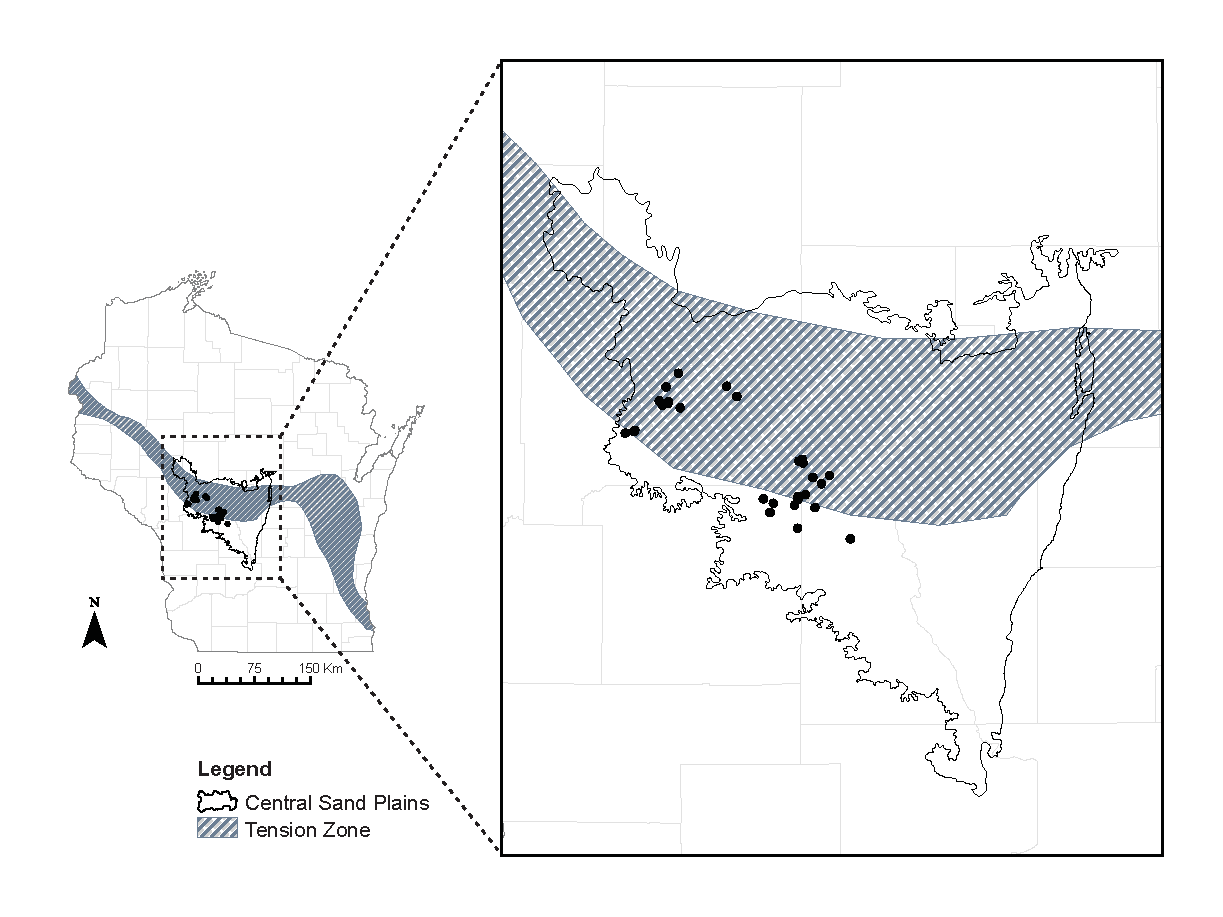
\includegraphics[width=0.9\textwidth]{chapter1/figures-maintext/map_20140214.pdf}\caption{\label{fig:Reampled-sites-in} Map of the 30 study sites in the central sand plains of Wisconsin.}
\end{figure}


\clearpage{}

\appendix

%\newcommand{\tablename0}{\tablename}
%\newcommand{\thetable0}{\thetable}
%\newcommand{\figurename0}{\figurename}
%\newcommand{\thefigure0}{\thefigure}
\renewcommand{\tablename}{\textsc{Table}}
\renewcommand {\thetable}{\textbf{A\arabic{table}}}
\renewcommand{\figurename}{\textsc{Fig.}}
\renewcommand {\thefigure}{\textbf{A\arabic{figure}}}
\setcounter{figure}{0}
\setcounter{table}{0}

\setlength{\tabcolsep}{2pt}
\LTcapwidth=\textwidth

\begin{onehalfspace}
\begin{longtable}[h]{p{0.02\textwidth}p{0.35\textwidth}p{0.1\textwidth}p{0.1\textwidth}p{0.1\textwidth}p{0.1\textwidth}p{0.15\textwidth}}
\caption{Results of indicator species analysis.}\\

\toprule

 & Taxon & Site \#(1958) & Site \#(2012) & Quadrat \%(1958) & Quadrat \%(2012) & Status\\
 \hline
\endfirsthead
\hline
& Taxon & Site \#(1958) & Site \#(2012) & Quadrat \%(1958) & Quadrat \%(2012) & Status\\
\hline
 \endhead
 \hline
\multicolumn{7}{r}{continued in next page\dots} \\
\endfoot
\bottomrule
\endlastfoot

1 & \emph{Acer rubrum } &  21 &  30 & 31.67 & 63.87 & winner \\
  2 & \emph{Achillea millefolium } &   7 &   1 & 1.67 & 0.07 & loser \\
  3 & \emph{Amelanchier spp } &  14 &  23 & 5.00 & 8.27 & winner \\
  4 & \emph{Andropogon gerardii } &   6 &   1 & 4.83 & 0.53 & not change \\
  5 & \emph{Anemone quinquefolia}  &   3 &   9 & 0.83 & 2.93 & winner \\
  6 & \emph{Antennaria spp } &  12 &   1 & 5.33 & 0.07 & loser \\
  7 & \emph{Apocynum androsaemifolium } &  18 &  18 & 6.17 & 4.67 & not change \\
  8 & \emph{Aralia nudicaulis } &  13 &  14 & 8.33 & 3.53 & not change \\
  9 & \emph{Arctostaphylos uva-ursi}  &   3 &   1 & 1.50 & 0.07 & not change \\
  10 & \emph{Aronia melanocarpa}  &   0 &  22 & 0.00 & 10.00 & winner \\
  \end{longtable}
\end{onehalfspace}

\begin{figure}
\begin{centering}
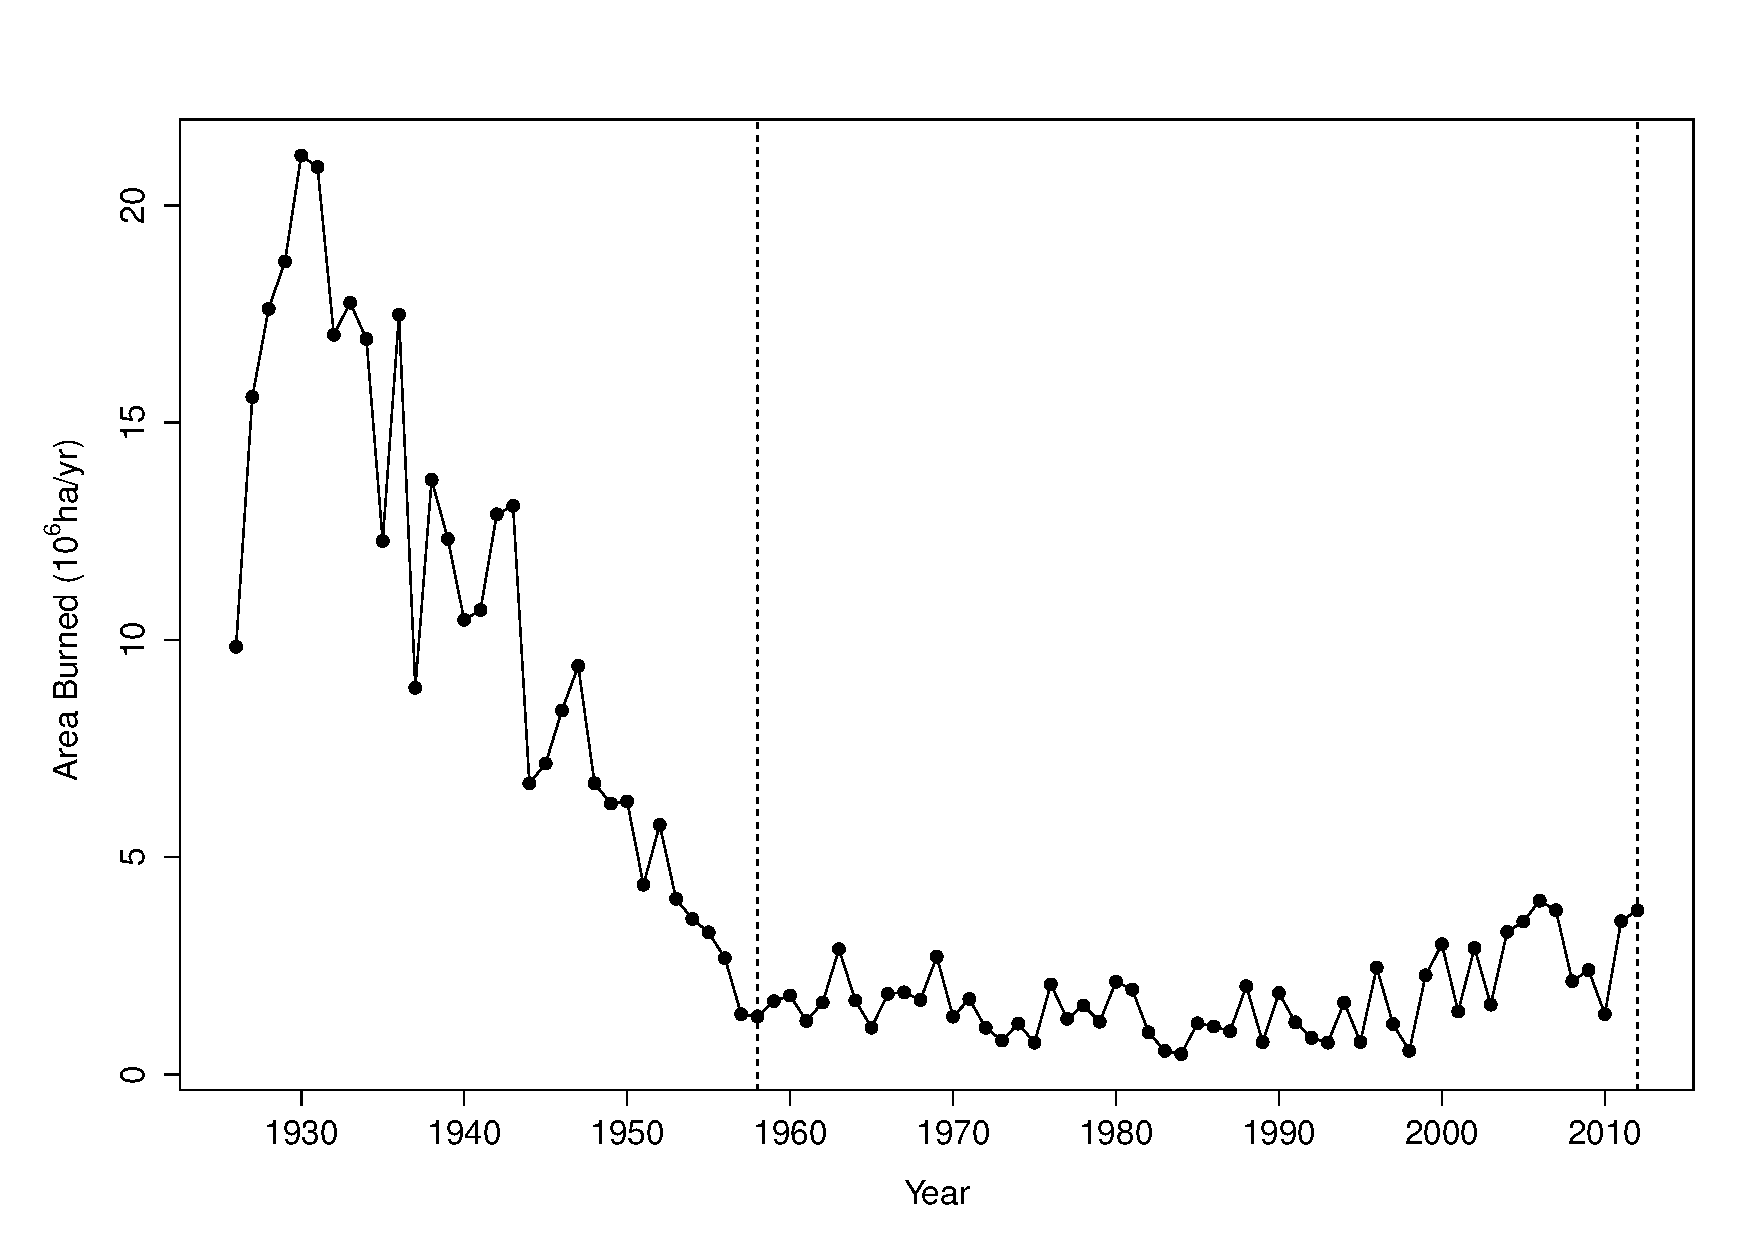
\includegraphics[width=1\textwidth]{chapter1/figures-appendix/fire.pdf}
\par\end{centering}
\caption{\label{fig:Fire-burning-extent}Fire burning extent in the United
States in millions of hectares per year from 1926 to 2012.}
\end{figure}

% so next chapter's figure/table names will be normal
\renewcommand{\tablename}{Table}
\renewcommand{\thetable}{\arabic{table}}
\renewcommand{\figurename}{Figure}
\renewcommand{\thefigure}{\arabic{figure}}
\clearpage

\clearpage
\phantomsection
% \addcontentsline{toc}{chapter}{Chapter 2 -- chapter one title here}
\cftaddtitleline{toc}{chapter}{Chapter 2 -- chapter one title here}{10}

\resetlinenumber

\begin{center}
\textbf{\Large{}Chapter 2 -- chapter one title here}
\label{chap:chapter2}
\par\end{center}{\Large \par}

\bigskip{}


\begin{center}
Your name\textsuperscript{*} and Your advisor
\par\end{center}

\bigskip{}

\lyxaddress{Department of Botany, University of Wisconsin-Madison, Madison, WI,
53706 USA}

Emails: xxx@wisc.edu

{*} Correspondence: Your name, Tel: (608) 265-2191

\chapter*{}
\setcounter{chapter}{2}


\textbf{Abstract:}

Plant community functional traits allow us to mechanistically link changes in species composition to changes in ecosystem functions.

\textbf{\emph{Keywords:}} long-term community assembly; functional
diversity.

\clearpage{}

\phantomsection\addcontentsline{toc}{section}{Introduction}
\section*{Introduction}

Global biodiversity is changing at an unprecedented rate in response to ongoing anthropogenic global environmental changes \citep{sala2000biodiversity}.

\phantomsection\addcontentsline{toc}{section}{Methods}
\section*{Methods}
\subsection*{Study sites and vegetation data}
We re-sampled 30 sites in the central sand plains (CSP) of Wisconsin in 2012 first sampled by James Habeck in 1958.

\phantomsection\addcontentsline{toc}{section}{Results}
\section*{Results}
\subsection*{Changes in environmental conditions}
Both stand characteristics and climatic conditions have changed since 1958. Average canopy cover, average annual precipitation, average annual temperature, and average temperature of the coldest month in these communities have all increased (Fig. \ref{fig:shade_climate_changes}, paired t-tests, all $p\ll0.001$).

\phantomsection\addcontentsline{toc}{section}{Discussion}
\section*{Discussion}
Widespread changes in disturbance regimes make it critical to understand the long-term impacts of disturbance on the taxonomic and functional diversity of plant communities.

\phantomsection\addcontentsline{toc}{section}{Conclusions}
\section*{Conclusions}
These pine barrens communities have increased in local functional diversity while converging in functional composition across sites.

\subsection*{Acknowledgments }
We thank James R. Habeck for his original sampling effort.

\clearpage{}
% \nocite{*}
\begin{onehalfspace}
\phantomsection\addcontentsline{toc}{section}{References}
\bibliographystyle{ecology}
\bibliography{chapter2/ch2}
\end{onehalfspace}

\clearpage{}

\setcounter{table}{0}
\setcounter{figure}{0}

\phantomsection\addcontentsline{toc}{section}{Tables}
\section*{Tables:}
\vspace{60pt}
\begin{table}[h]
\caption{\label{tab:functional-traits-list}List of functional traits used
in this study.}


\centering{}%
\begin{tabular}{>{\raggedright}p{0.2\textwidth}>{\raggedright}p{0.3\textwidth}>{\raggedright}p{0.3\textwidth}>{\raggedright}p{0.2\textwidth}}

\toprule
Trait (Abb.) & Description & Related function & Life-cycle phase\tabularnewline
\midrule
{\small{}Pollination mode (Biotic.Polli)} & {\small{}Biotic or Abiotic} & {\small{}Regeneration strategy} & \emph{\small{}Regeneration}\tabularnewline
{\small{}Leaf nitrogen concentration (LNC)} & {\small{}Total amount of nitrogen per unit of leaf dry mass (\%)} & {\small{}Light capture, photosynthetic rate} & \emph{\small{}Vegetative growth}\tabularnewline
\bottomrule
\end{tabular}
\end{table}

\clearpage{}
\phantomsection\addcontentsline{toc}{section}{Figures}
\noindent\textbf{Figures:}

\noindent \textbf{Figure 1.} Changes in canopy cover, annual average temperature, average temperature of coldest month, and annual precipitation of study sites over time.
\clearpage{}


\begin{figure}
\begin{centering}
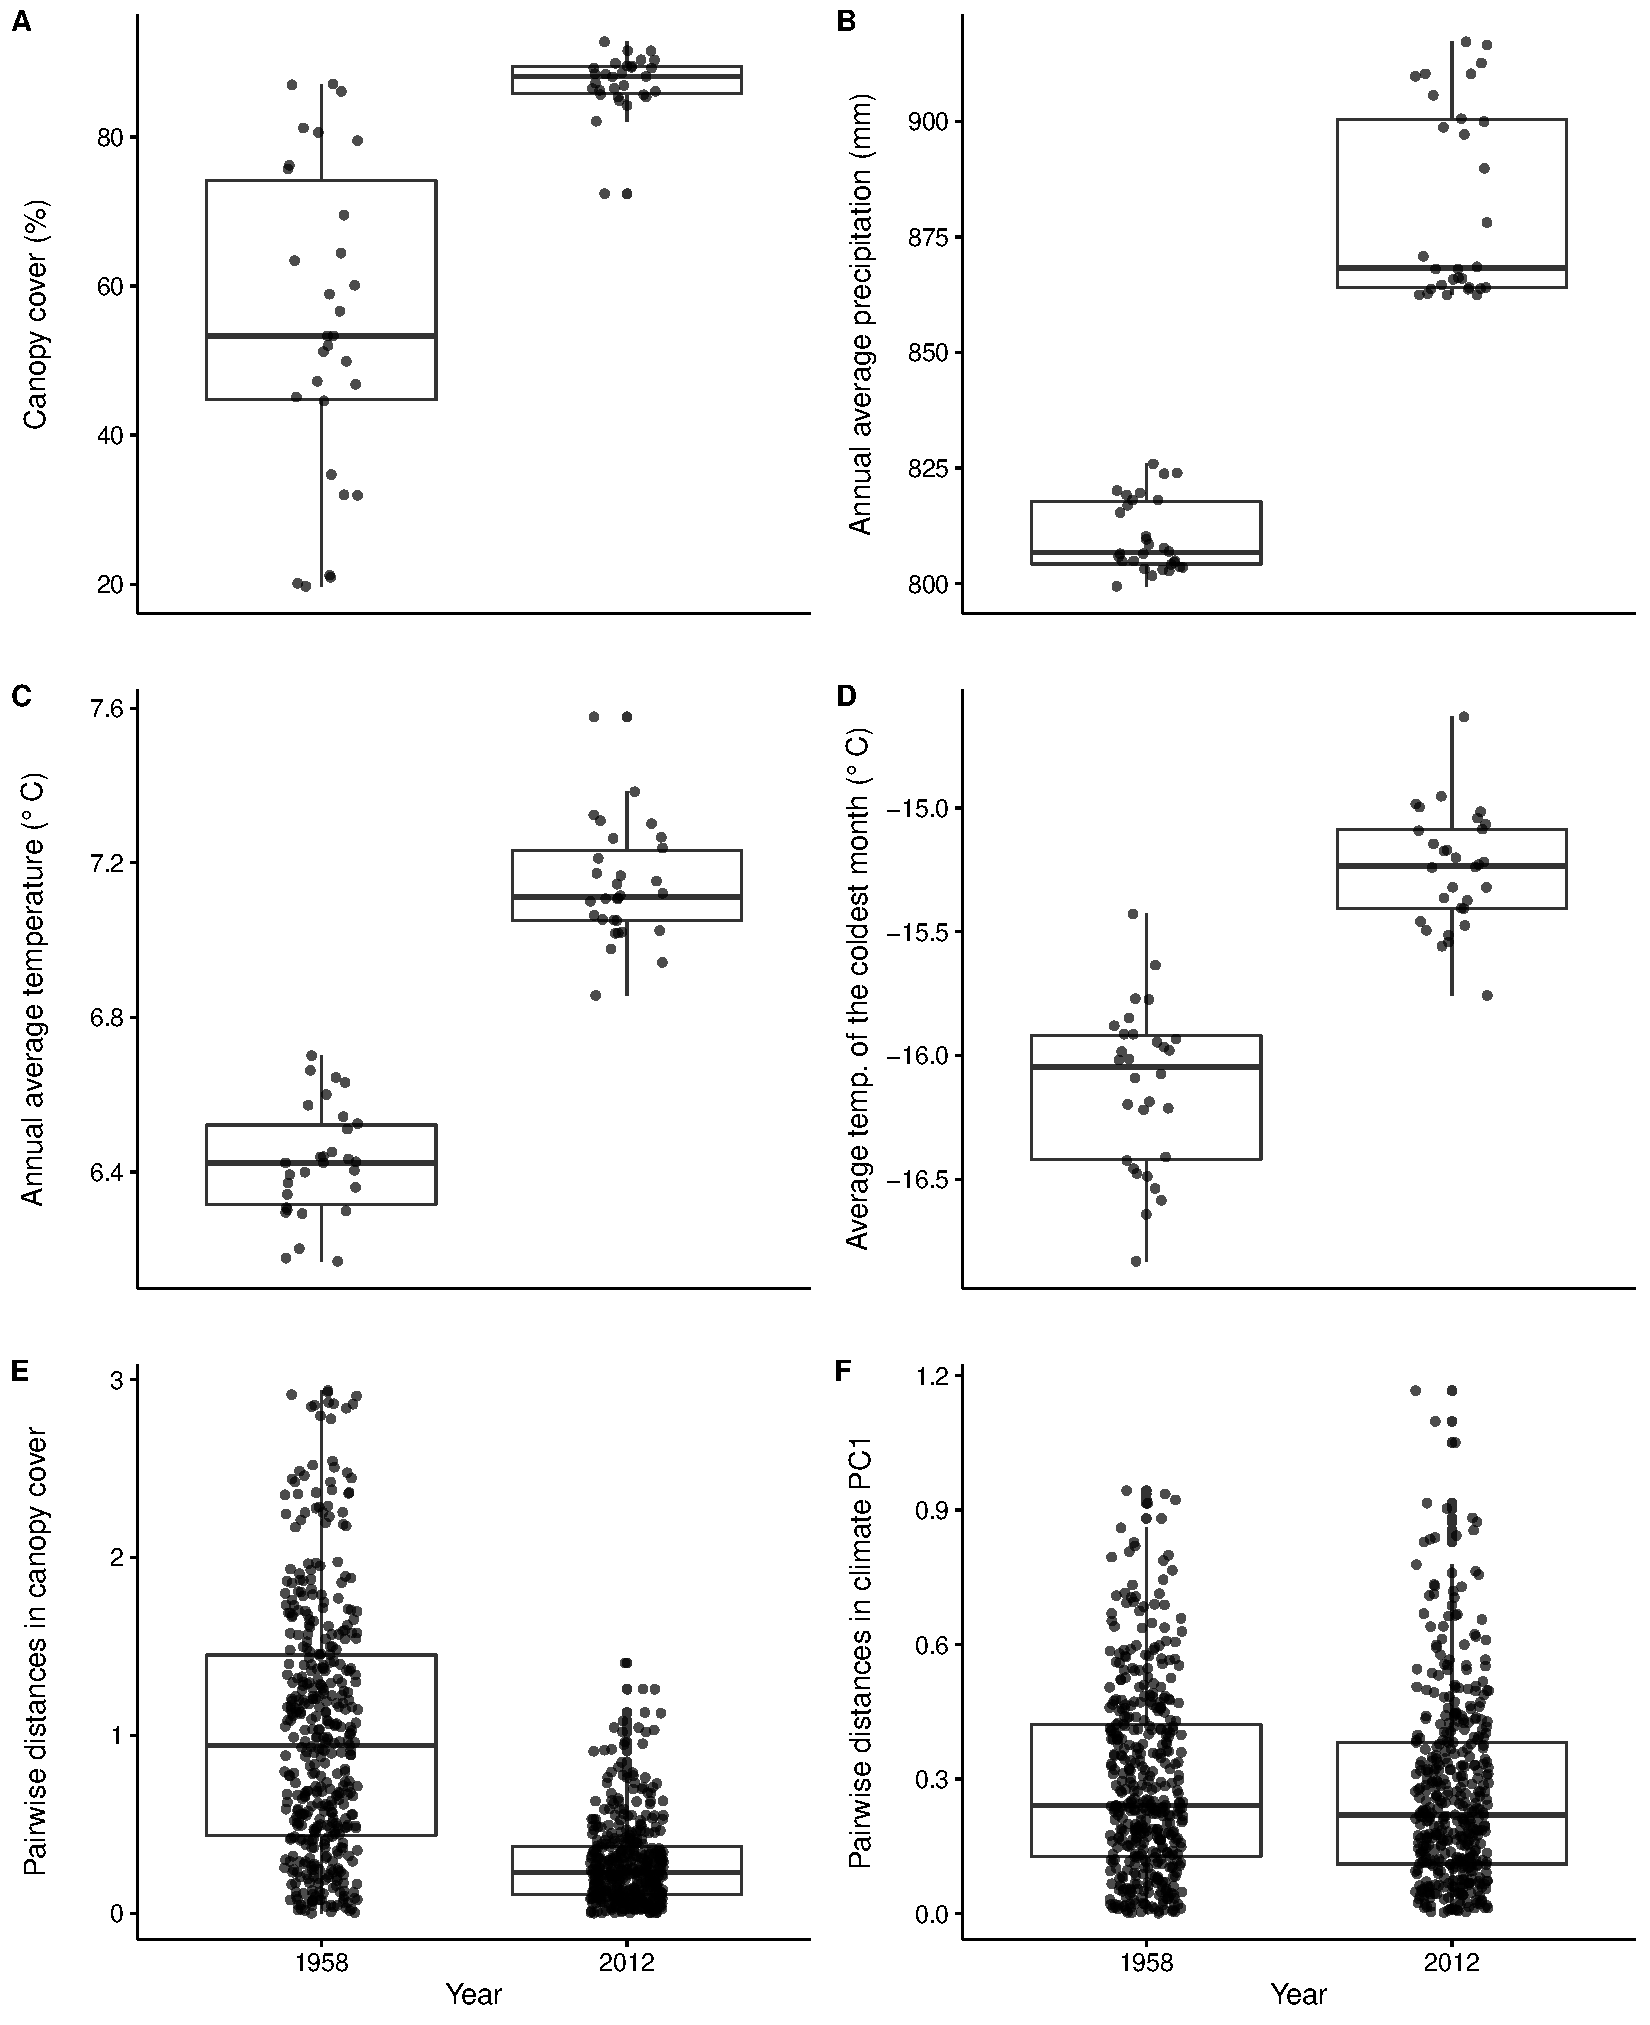
\includegraphics[width=1\textwidth]{chapter2/figures-maintext/shade_climate.pdf}
\par\end{centering}
\caption{\label{fig:shade_climate_changes}
}
\end{figure}

\clearpage{}

\appendix  %%% Appendix %%%%%%%%%%%%%%%%%%%%%%%%%%%%%%%%%%%%%%%%

\renewcommand{\tablename}{\textsc{Table}}
\renewcommand {\thetable}{\textbf{A\arabic{table}}}
\renewcommand{\figurename}{\textsc{Fig.}}
\renewcommand {\thefigure}{\textbf{A\arabic{figure}}}
\setcounter{figure}{0}
\setcounter{table}{0}
\phantomsection\addcontentsline{toc}{section}{Appendix}
\textbf{\LARGE{}Appendix}{\LARGE{}: Supplementary materials.}{\LARGE \par}

\bigskip{}


\textbf{Text A1:} Cumulative proportions and loading of PCA based
on eight climatic variables.\\

\begin{onehalfspace}
\begin{knitrout}
\definecolor{shadecolor}{rgb}{0.969, 0.969, 0.969}\color{fgcolor}\begin{kframe}
\begin{alltt}
\hlkwd{summary}\hlstd{(climate.pca)}
\end{alltt}
\begin{verbatim}
## Importance of components:
##                           PC1     PC2    PC3     PC4    PC5     PC6
## Standard deviation     2.5629 0.88087 0.6499 0.45706 0.1358 0.06558
## Proportion of Variance 0.8211 0.09699 0.0528 0.02611 0.0023 0.00054
## Cumulative Proportion  0.8211 0.91807 0.9709 0.99698 0.9993 0.99982
##                            PC7     PC8
## Standard deviation     0.03344 0.01825
## Proportion of Variance 0.00014 0.00004
## Cumulative Proportion  0.99996 1.00000
\end{verbatim}
\end{knitrout}
\end{onehalfspace}

\begin{figure}
\begin{centering}
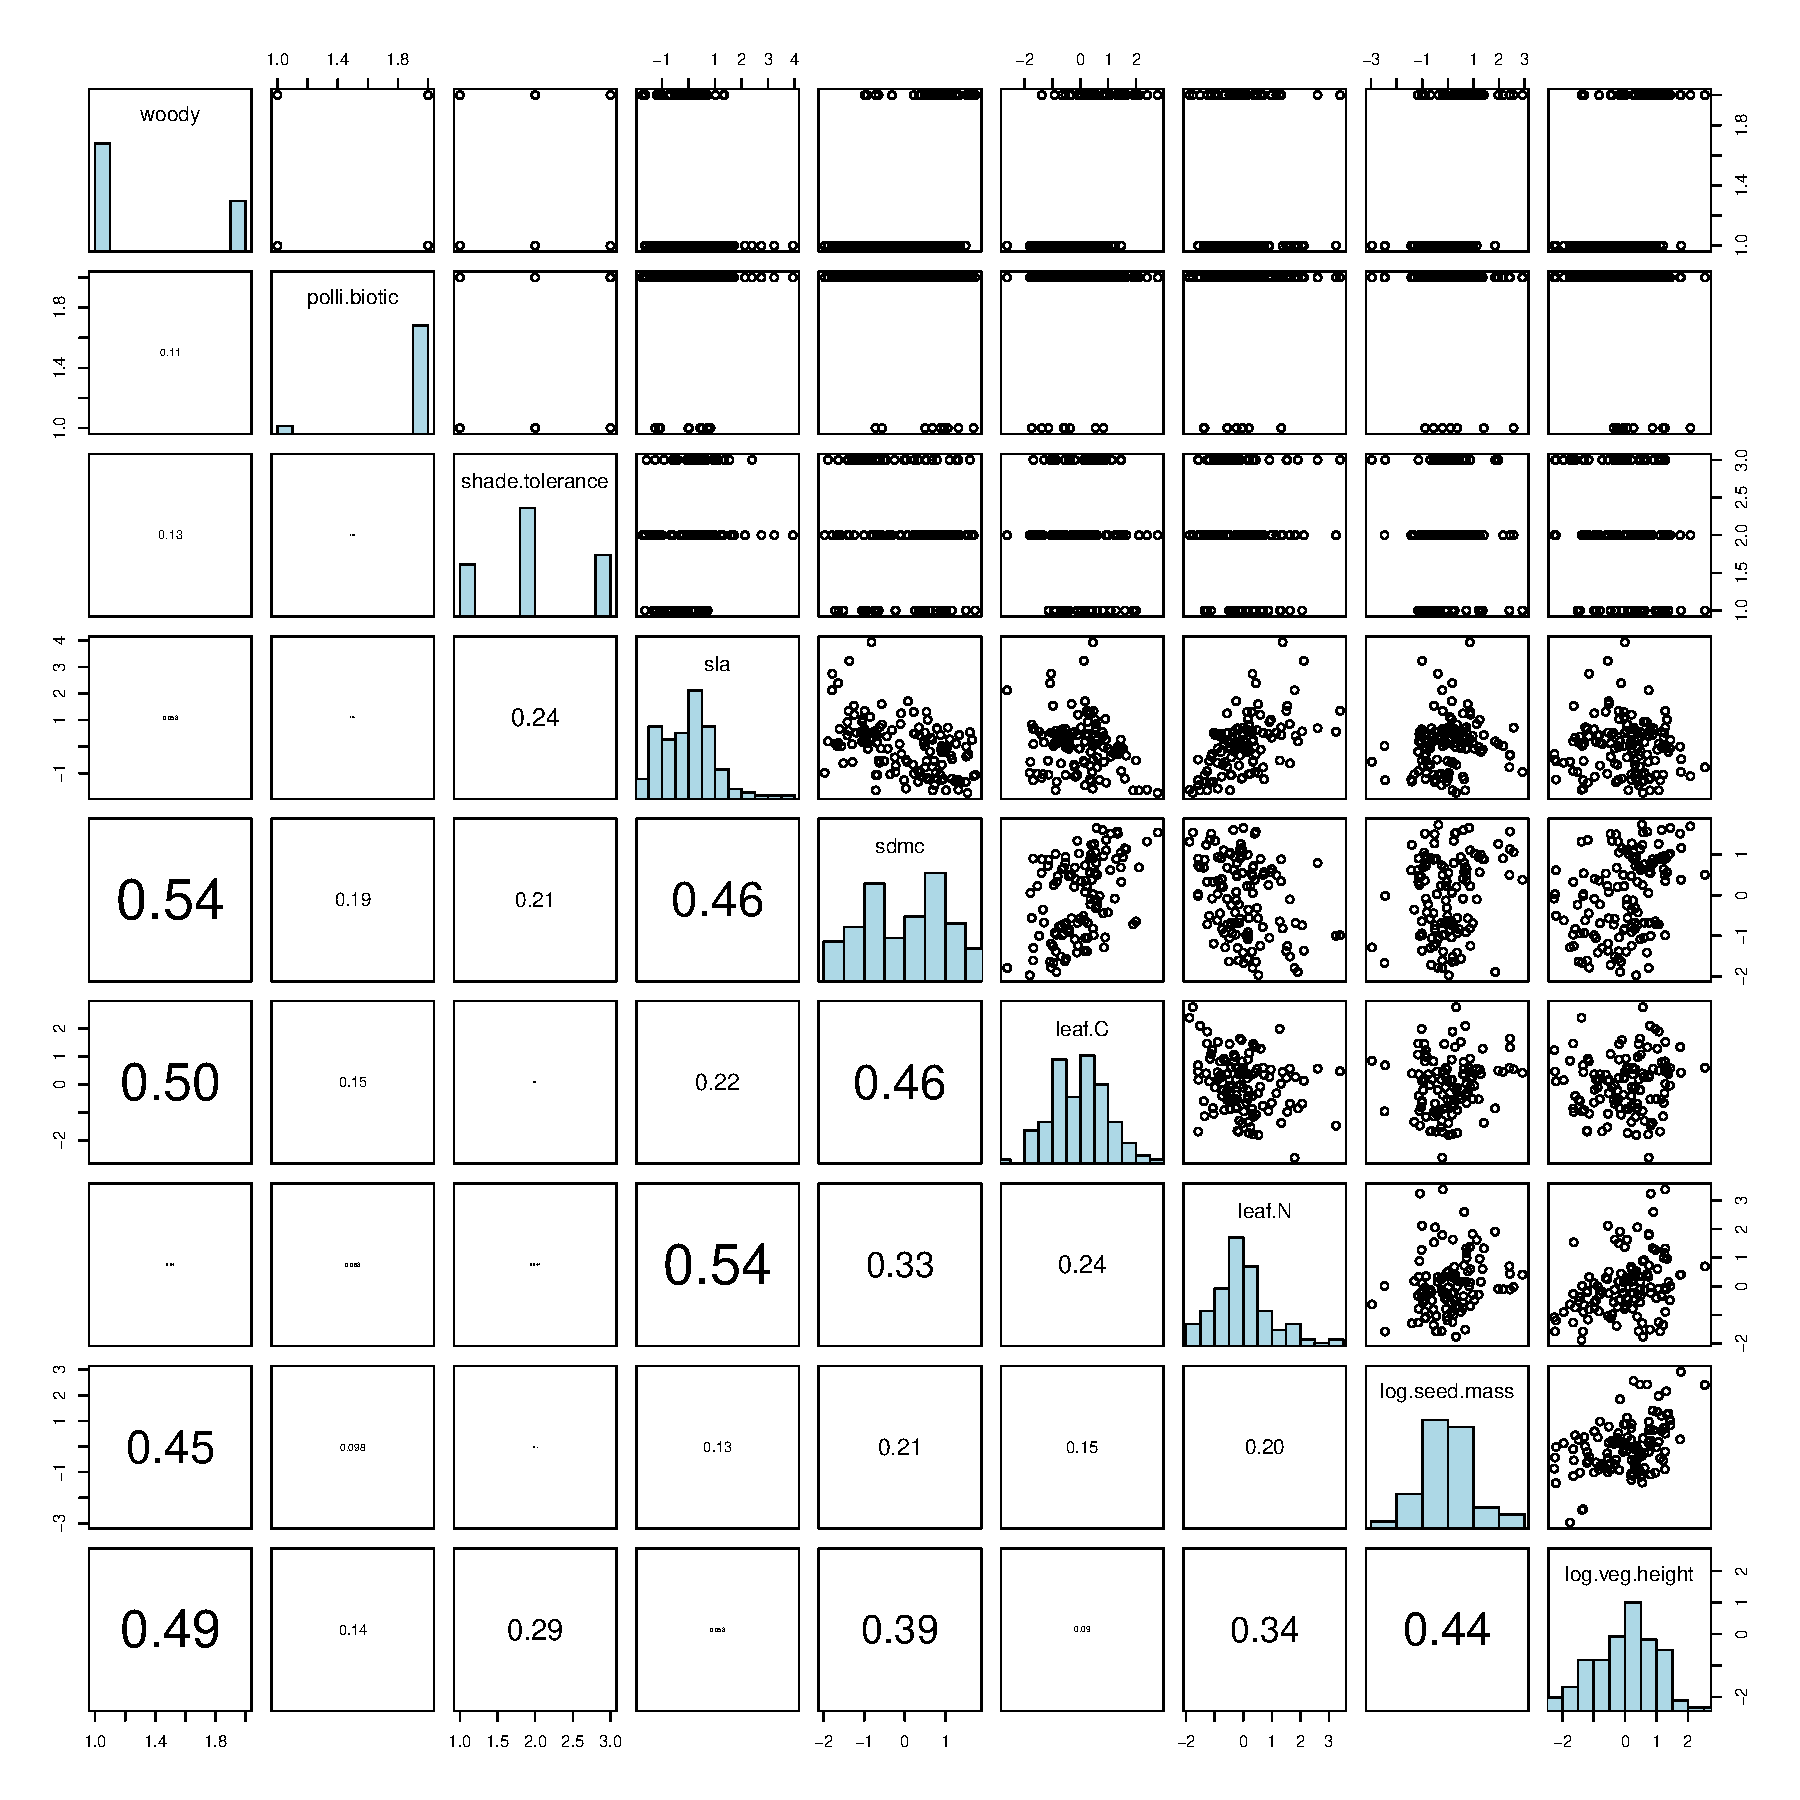
\includegraphics[width=1\textwidth]{chapter2/figures-appendix/trait_cor.pdf}
\par\end{centering}
\caption{Distribution of functional traits used in this study and their pairwise correlations (in absolute value).}
\end{figure}

\renewcommand{\tablename}{Table}
\renewcommand{\thetable}{\arabic{table}}
\renewcommand{\figurename}{Figure}
\renewcommand{\thefigure}{\arabic{figure}}


\clearpage{}


\end{document}
